\documentclass[12pt,a4paper]{article}

\usepackage[utf8]{inputenc}
\usepackage[T1]{fontenc}
\usepackage[spanish,es-noquoting]{babel}
\usepackage{amsmath, amssymb}
\usepackage[top=2.5cm, bottom=2.5cm, left=3cm, right=2.5cm, headheight=14pt]{geometry}
\usepackage{booktabs}
\usepackage{array}
\usepackage{graphicx}
\usepackage{hyperref}
\usepackage{xcolor}
\usepackage{enumitem}
\usepackage{fancyhdr}
\usepackage{titlesec}

\definecolor{accent}{RGB}{30, 80, 160}

\hypersetup{
    colorlinks=true,
    linkcolor=accent,
    urlcolor=accent,
    pdftitle={Entrega Parcial -- Metricas de Centralidad en Redes}
}

\pagestyle{fancy}
\fancyhf{}
\rhead{\small Proyecto Semestral -- Estructuras de Datos}
\lhead{\small Métricas de Centralidad en Redes}
\cfoot{\thepage}
\renewcommand{\headrulewidth}{0.4pt}

\titleformat{\section}{\large\bfseries\color{accent}}{}{0em}{}[\titlerule]
\titleformat{\subsection}{\normalsize\bfseries}{}{0em}{}

\setlength{\parskip}{6pt}
\setlength{\parindent}{0pt}

% ─────────────────────────────────────────────
\begin{document}

% ── PORTADA ──────────────────────────────────
\begin{titlepage}
    \centering
    \vspace*{1.5cm}

    {\large \textbf{Universidad --- Ingeniería en Computación}}\\[0.3cm]
    {\large Estructuras de Datos}\\[2cm]

    \noindent\rule{\linewidth}{1pt}\\[0.4cm]
    {\LARGE \textbf{Entrega Parcial}}\\[0.3cm]
    {\Large Métricas de Centralidad en Redes}\\[0.3cm]
    \noindent\rule{\linewidth}{1pt}\\[2cm]

    \begin{tabular}{ll}
        \textbf{Integrante 1:} & Nicolás Ricciardi \\[0.4cm]
        \textbf{Integrante 2:} & Enzo Levancini \\[0.4cm]
        \textbf{Integrante 3:} & Máximo Beltrán \\[0.4cm]
    \end{tabular}

    \vfill
    {\large Junio 2026}
\end{titlepage}

% ── INDICE ───────────────────────────────────
\tableofcontents
\newpage

\section{Introducción}

Una \textbf{red} es una estructura matemática compuesta por un conjunto de \textbf{vértices}
(nodos) y un conjunto de \textbf{aristas} (relaciones entre nodos). Formalmente, un grafo
$G = (V, E)$ donde $V$ es el conjunto de vértices y $E \subseteq V \times V$ el de aristas.

Las redes aparecen de forma natural en muchos dominios:

\begin{center}
\begin{tabular}{lll}
\toprule
\textbf{Dominio} & \textbf{Vértice} & \textbf{Arista} \\
\midrule
Biología & Proteína & Interacción física \\
Comercio & País & Flujo comercial \\
Cine & Actor & Aparición en la misma película \\
Informática & Dirección IP & Conexión de red \\
\bottomrule
\end{tabular}
\end{center}

Una pregunta central en el análisis de redes es: \textit{¿cuál elemento es el más
``importante''?} La respuesta depende de qué se entiende por importancia. Las
\textbf{métricas de centralidad} responden esta pregunta desde distintos ángulos,
cada una capturando una noción diferente de relevancia estructural.

En este proyecto se implementan \textbf{siete métricas de centralidad}, aplicadas
sobre dos redes reales: la red de interacciones proteína-proteína de levadura (\textit{Yeast PPI})
y la red de comercio internacional (\textit{Trade Network}).

\section{Métricas de Centralidad}

\subsection{Degree Centrality}

\textbf{Concepto.} Un vértice es importante si tiene muchas conexiones directas.
Es la métrica más simple y sirve como referencia para comparar con las demás.

\textbf{Fórmula} (grafo no dirigido, normalizada):
\[
C_D(v) = \frac{\deg(v)}{n - 1}
\]
donde $\deg(v)$ es el número de vecinos directos de $v$ y $n = |V|$.

En grafos \textbf{dirigidos} se distingue in-degree (aristas entrantes, popularidad)
y out-degree (aristas salientes, actividad).

\textbf{Complejidad:} $O(|V| + |E|)$

\textbf{Aplicación.} En la red Yeast PPI, una proteína con alto degree es un
\textit{hub} biológico cuya eliminación puede resultar letal para el organismo.
En Trade Network, el in-degree refleja diversificación de importaciones y el
out-degree el alcance exportador de un país.

% ────────────────────────────────────────────────
\subsection{Betweenness Centrality}

\textbf{Concepto.} Un vértice es importante si actúa como puente en los caminos
más cortos entre otros pares. Captura el control sobre el flujo en la red.

\textbf{Fórmula:}
\[
C_B(v) = \sum_{\substack{s \neq v \neq t \\ s \neq t}}
         \frac{\sigma_{st}(v)}{\sigma_{st}}
\]
donde $\sigma_{st}$ es el número total de caminos más cortos entre $s$ y $t$,
y $\sigma_{st}(v)$ los que pasan por $v$.

\textbf{Normalización:}
\[
C_B^{\text{norm}}(v) =
\begin{cases}
\dfrac{C_B(v)}{(n-1)(n-2)} & \text{dirigido} \\[8pt]
\dfrac{2\,C_B(v)}{(n-1)(n-2)} & \text{no dirigido}
\end{cases}
\]

\textbf{Algoritmo:} Brandes~\cite{brandes2001}, que calcula la betweenness exacta
para todos los vértices con un BFS por vértice fuente.

\textbf{Complejidad:} $O(|V| \cdot |E|)$

\textbf{Aplicación.} En Yeast PPI, alta betweenness indica proteínas que conectan
módulos funcionales distintos; su eliminación puede desconectar regiones de la red.
En Trade Network, identifica países que actúan como intermediarios críticos del
comercio global.

% ────────────────────────────────────────────────
\subsection{Closeness Centrality}

\textbf{Concepto.} Un vértice es importante si puede alcanzar rápidamente a todos
los demás. Se basa en la inversa de la distancia promedio.

\textbf{Fórmula} (Wasserman \& Faust~\cite{wasserman1994}, para grafos desconectados):
\[
C_C(v) = \frac{n-1}{N-1} \cdot \frac{n-1}{\displaystyle\sum_{u \neq v} d(v,u)}
\]
donde $n$ es el número de vértices alcanzables desde $v$, $N = |V|$ el total,
y $d(v,u)$ la distancia mínima entre $v$ y $u$.

El factor $\frac{n-1}{N-1}$ penaliza vértices que no alcanzan al resto, permitiendo
comparar en grafos desconectados.

\textbf{Complejidad:} $O(|V| \cdot (|V|+|E|))$ via BFS desde cada vértice.

\textbf{Aplicación.} En Yeast PPI, alta closeness indica proteínas con rol
regulatorio global, capaces de transmitir señales al resto de la red en pocas
interacciones. En Trade Network, países con alta closeness están integrados
eficientemente con la economía mundial.

% ────────────────────────────────────────────────
\subsection{PageRank}

\textbf{Concepto.} Un vértice es importante si está conectado a otros vértices
importantes. Un enlace desde un nodo de alto PageRank vale más~\cite{pagerank1999}.

\textbf{Fórmula iterativa:}
\[
PR(v) = \frac{1-d}{n} + d \sum_{u \in N^{-}(v)} \frac{PR(u)}{|N^{+}(u)|}
\]
donde $d = 0.85$ es el factor de amortiguación (\textit{damping factor}),
$N^{-}(v)$ son los vecinos que apuntan a $v$, y $N^{+}(u)$ los destinos de $u$.

El término $\frac{1-d}{n}$ modela la probabilidad de salto aleatorio a cualquier nodo.
El algoritmo itera hasta convergencia ($\|PR^{(k+1)} - PR^{(k)}\|_1 < 10^{-6}$).

\textbf{Complejidad:} $O(k \cdot (|V|+|E|))$, con $k < 100$ en la práctica.

\textbf{Aplicación.} En Trade Network, el PageRank refleja la importancia de un
país en el comercio global ponderada por la importancia de sus socios, capturando
influencia indirecta que el degree no detecta. En Yeast PPI, identifica proteínas
centrales cuya importancia está reforzada por sus vecinas.

% ────────────────────────────────────────────────
\subsection{Average Shortest Path}

\textbf{Concepto.} Promedio de las distancias mínimas desde un vértice hacia todos
los demás alcanzables. Un valor alto indica aislamiento estructural.

\textbf{Fórmula por vértice:}
\[
ASP(v) = \frac{1}{|R(v)|} \sum_{u \in R(v)} d(v, u)
\]
donde $R(v)$ son los vértices alcanzables desde $v$ (excluyendo $v$).

\textbf{Métrica global:}
\[
\overline{ASP} = \frac{1}{|V|} \sum_{v \in V} ASP(v)
\]
Esta métrica global cuantifica la compacidad de la red entera. El experimento de
los \textit{seis grados de separación} corresponde a medir $\overline{ASP}$ en la
red social humana.

\textbf{Complejidad:} $O(|V| \cdot (|V|+|E|))$

\textbf{Aplicación.} En Yeast PPI, un $\overline{ASP}$ bajo confirma que la red
es compacta (propiedad de \textit{small-world}), lo que facilita la propagación
de señales biológicas. En Trade Network, países con bajo $ASP$ individual son los
más integrados al sistema de comercio global.

% ────────────────────────────────────────────────
\subsection{Eigenvector Centrality}

\textbf{Concepto.} Extiende el degree ponderando cada vecino por su propia
centralidad. Es la base matemática del PageRank~\cite{bonacich1987}.

\textbf{Definición.} Sea $\mathbf{A}$ la matriz de adyacencia. El vector
$\mathbf{x}$ de Eigenvector Centrality satisface:
\[
\mathbf{A}\,\mathbf{x} = \lambda\,\mathbf{x}
\qquad \Longleftrightarrow \qquad
C_E(v) = \frac{1}{\lambda} \sum_{u \in N(v)} C_E(u)
\]
donde $\lambda$ es el autovalor dominante de $\mathbf{A}$ (Perron-Frobenius).

\textbf{Algoritmo:} \textit{Power Iteration}: inicializar $\mathbf{x}^{(0)}$
uniformemente, iterar $\mathbf{x}^{(k+1)} \leftarrow \mathbf{A}\,\mathbf{x}^{(k)}$
normalizando por el máximo hasta convergencia.

\textbf{Complejidad:} $O(k \cdot (|V|+|E|))$

\textbf{Diferencia con PageRank.} PageRank agrega un factor de amortiguación $d$ y
maneja nodos sin salidas. Eigenvector Centrality es la versión pura; ambos coinciden
cuando $d \to 1$ y no hay nodos dangling.

\textbf{Aplicación.} En Yeast PPI, identifica el núcleo funcional: proteínas que
interactúan con otras que también son muy conectadas. En Trade Network, captura países
cuya influencia comercial se amplifica por sus socios.

% ────────────────────────────────────────────────
\subsection{Clustering Coefficient}

\textbf{Concepto.} Mide qué fracción de los vecinos de un vértice están conectados
entre sí. Cuantifica la tendencia a formar grupos locales (\textit{clustering})~\cite{watts1998}.

\textbf{Fórmula local:}
\[
C_{Cl}(v) = \frac{|\{(u,w) \in E \;:\; u,w \in N(v)\}|}{\deg(v)\,(\deg(v)-1)}
\]
El numerador cuenta los pares de vecinos de $v$ que están conectados (triángulos
que pasan por $v$); el denominador es el máximo posible. El resultado está en $[0,1]$.

\textbf{Coeficiente global:}
\[
\overline{C_{Cl}} = \frac{1}{|V|} \sum_{v \in V} C_{Cl}(v)
\]

\textbf{Complejidad:} $O(|V| \cdot \overline{\deg}^{\,2})$, donde $\overline{\deg}$ es el grado promedio.

\textbf{Aplicación.} En Yeast PPI, alto clustering indica la presencia de complejos
proteicos: grupos donde todas las proteínas interactúan entre sí (ribosomas, complejos
de transcripción). En Trade Network, alto clustering de un país indica que sus socios
comerciales también comercian entre sí, formando bloques económicos regionales.

\section{Datasets Seleccionados}

\subsection{Dataset 1: Yeast Protein-Protein Interaction Network}

\begin{center}
\begin{tabular}{ll}
\toprule
\textbf{Característica} & \textbf{Valor} \\
\midrule
Tipo & No dirigido, no ponderado \\
Vértices & 6.526 proteínas \\
Aristas & 532.180 interacciones \\
Formato & Lista de aristas separada por tabuladores \\
Fuente & Kaggle / Alexander Chervov \\
\bottomrule
\end{tabular}
\end{center}

Cada fila representa una interacción entre dos proteínas identificadas por sus nombres
sistemáticos (e.g., \texttt{YLR418C}, \texttt{YOL145C}). El archivo lista cada arista
en ambas direcciones, por lo que se aplica deduplicación durante la carga.

Las proteínas de \textit{Saccharomyces cerevisiae} son ampliamente usadas como
organismo modelo en biología celular. Esta red es un benchmark clásico en análisis
de redes biológicas.

\subsection{Dataset 2: Trade Network}

\begin{center}
\begin{tabular}{ll}
\toprule
\textbf{Característica} & \textbf{Valor} \\
\midrule
Tipo & Dirigido, ponderado \\
Vértices & $\approx$ 161 países \\
Aristas & Miles de relaciones comerciales \\
Peso de arista & Valor del flujo comercial (USD) \\
Formato & Pajek \texttt{.net} \\
Años disponibles & 2000, 2005, 2010, 2015, 2018 \\
\bottomrule
\end{tabular}
\end{center}

El archivo Pajek contiene una sección \texttt{*Vertices} con países y coordenadas,
seguida de \texttt{*Arcs} con las exportaciones dirigidas y su peso en USD.
Una arista $A \to B$ con peso $w$ indica que el país $A$ exportó $w$ USD al país $B$.

Para los experimentos se combinan los cinco años en un único grafo, conservando
el peso máximo observado para cada par de países. Esto produce la red de comercio
internacional más completa del dataset.

\section{Análisis de Complejidad Teórica}

\subsection{Representación: Lista de Adyacencia}

Se utiliza una lista de adyacencia implementada con \texttt{unordered\_map<int, vector<Edge>>}.
Esta representación es óptima para redes reales, que son típicamente dispersas ($|E| \ll |V|^2$)~\cite{cormen2009}.

\begin{center}
\begin{tabular}{lccc}
\toprule
\textbf{Representación} & \textbf{Memoria} & \textbf{Iterar vecinos} & \textbf{Verificar arista} \\
\midrule
Lista de adyacencia & $O(|V|+|E|)$ & $O(\deg(v))$ & $O(\deg(v))$ \\
Matriz de adyacencia & $O(|V|^2)$ & $O(|V|)$ & $O(1)$ \\
\bottomrule
\end{tabular}
\end{center}

Para Yeast con $|V| = 6.526$, una matriz requeriría $6.526^2 \approx 42$ millones de
entradas ($\sim 340$ MB), mientras que la lista de adyacencia ocupa $\sim 24$ MB.

\subsection{Operaciones sobre el Grafo}

\begin{center}
\begin{tabular}{lc}
\toprule
\textbf{Operación} & \textbf{Complejidad} \\
\midrule
\texttt{addVertex} & $O(1)$ esperado \\
\texttt{addEdge} & $O(1)$ esperado \\
\texttt{removeEdge} & $O(\deg(v))$ \\
\texttt{hasEdge} & $O(\deg(v))$ \\
Construcción completa & $O(|V|+|E|)$ \\
\bottomrule
\end{tabular}
\end{center}

\texttt{addVertex} inserta en \texttt{unordered\_map} y \texttt{addEdge} hace una búsqueda
en \texttt{unordered\_map} más un \texttt{push\_back} en \texttt{vector}. Ambas son $O(1)$
\textbf{esperado} (caso promedio con función de hash uniforme), no amortizado en el sentido
estricto: en el peor caso con colisiones degeneradas, la complejidad sube a $O(|V|)$.

\subsection{Complejidad de las Métricas}

\begin{center}
\begin{tabular}{lcc}
\toprule
\textbf{Métrica} & \textbf{Complejidad} & \textbf{Algoritmo base} \\
\midrule
Degree Centrality & $O(|V|+|E|)$ & Recorrido de vecinos \\
Betweenness Centrality & $O(|V| \cdot |E|)$ & Brandes (BFS por fuente) \\
Closeness Centrality & $O(|V| \cdot (|V|+|E|))$ & BFS por fuente \\
PageRank & $O(k \cdot (|V|+|E|))$ & Iteración de potencias \\
Average Shortest Path & $O(|V| \cdot (|V|+|E|))$ & BFS por fuente \\
Eigenvector Centrality & $O(k \cdot (|V|+|E|))$ & Power Iteration \\
Clustering Coefficient & $O(|V| \cdot \overline{\deg}^{\,2})$ & Conteo de triángulos \\
\bottomrule
\end{tabular}
\end{center}

donde $k$ es el número de iteraciones hasta convergencia ($k < 100$ en la práctica)
y $\overline{\deg}$ es el grado promedio de la red.

\textbf{Peor caso dominante:} Betweenness con $O(|V| \cdot |E|)$. Para Yeast esto
implica $6.526 \times 532.180 \approx 3{,}47 \times 10^9$ operaciones por ejecución,
lo que se verá reflejado en los experimentos.

\subsection{Relación entre Métricas}

Las métricas no son independientes. En redes reales existe correlación positiva entre
Degree y Eigenvector Centrality (hubs se conectan con hubs), mientras que Betweenness
puede identificar vértices con degree moderado pero posición estructural estratégica
(puentes entre comunidades). Esta comparación es parte del análisis experimental.

\section{Estudio Experimental}

\subsection{Metodología y Entorno de Pruebas}

Los experimentos se ejecutaron en un equipo con sistema operativo Windows 11 Home,
compilando con MinGW-w64 GCC 14.x en modo Release (optimización \texttt{-O2}).
Cada métrica se ejecutó \textbf{10 veces consecutivas} sobre el grafo ya construido
en memoria, reportando media aritmética, varianza, mínimo y máximo. La medición de
tiempo utiliza \texttt{std::chrono::high\_resolution\_clock}.

El código fuente está disponible en:
\url{https://github.com/ricachii/Centralidad-de-Redes}

\subsection{Construcción del Grafo}

\begin{center}
\begin{tabular}{lcc}
\toprule
\textbf{Dataset} & \textbf{Tiempo de construcción (ms)} & \textbf{Memoria (KB)} \\
\midrule
Yeast PPI (6.526V, 532.180E) & 3.902 & 24.150 \\
Trade Network (161V, 22.475E) & 551 & 571 \\
\bottomrule
\end{tabular}
\end{center}

La diferencia de memoria (24 MB vs 571 KB) refleja directamente el tamaño de cada red.
Usando lista de adyacencia, Yeast ocupa $\sim$24 MB frente a los $\sim$340 MB que
requeriría una matriz de adyacencia ($6.526^2$ entradas).

\subsection{Tiempo de Ejecución por Métrica}

\subsubsection*{Dataset 1: Yeast PPI}

\begin{center}
\begin{tabular}{lcccc}
\toprule
\textbf{Métrica} & \textbf{Media (ms)} & \textbf{Varianza (ms$^2$)} & \textbf{Mín} & \textbf{Máx} \\
\midrule
Degree Centrality     & 0{,}73      & 0{,}007    & 0{,}641   & 0{,}923  \\
PageRank              & 298         & 177        & 290       & 337      \\
Eigenvector           & 411         & 178        & 404       & 451      \\
Clustering Coeff.     & 10.493      & 341        & 10.459    & 10.514   \\
Closeness             & 60.020      & 3.365      & 59.903    & 60.128   \\
Average Shortest Path & 60.042      & 4.577      & 59.964    & 60.158   \\
Betweenness           & 109.452     & 87.823     & 109.039   & 110.020  \\
\bottomrule
\end{tabular}
\end{center}

\subsubsection*{Dataset 2: Trade Network}

\begin{center}
\begin{tabular}{lcccc}
\toprule
\textbf{Métrica} & \textbf{Media (ms)} & \textbf{Varianza (ms$^2$)} & \textbf{Mín} & \textbf{Máx} \\
\midrule
Degree Centrality     & 0{,}025 & $1{,}5\times10^{-5}$ & 0{,}020 & 0{,}032 \\
PageRank              & 24{,}9  & 0{,}18               & 24{,}3  & 25{,}7  \\
Eigenvector           & 34{,}5  & 0{,}049              & 34{,}3  & 34{,}9  \\
Clustering Coeff.     & 699     & 581                  & 666     & 727     \\
Closeness             & 705     & 735                  & 673     & 739     \\
Average Shortest Path & 702     & 644                  & 672     & 737     \\
Betweenness           & 722     & 1.602                & 647     & 786     \\
\bottomrule
\end{tabular}
\end{center}

\begin{figure}[h]
\centering
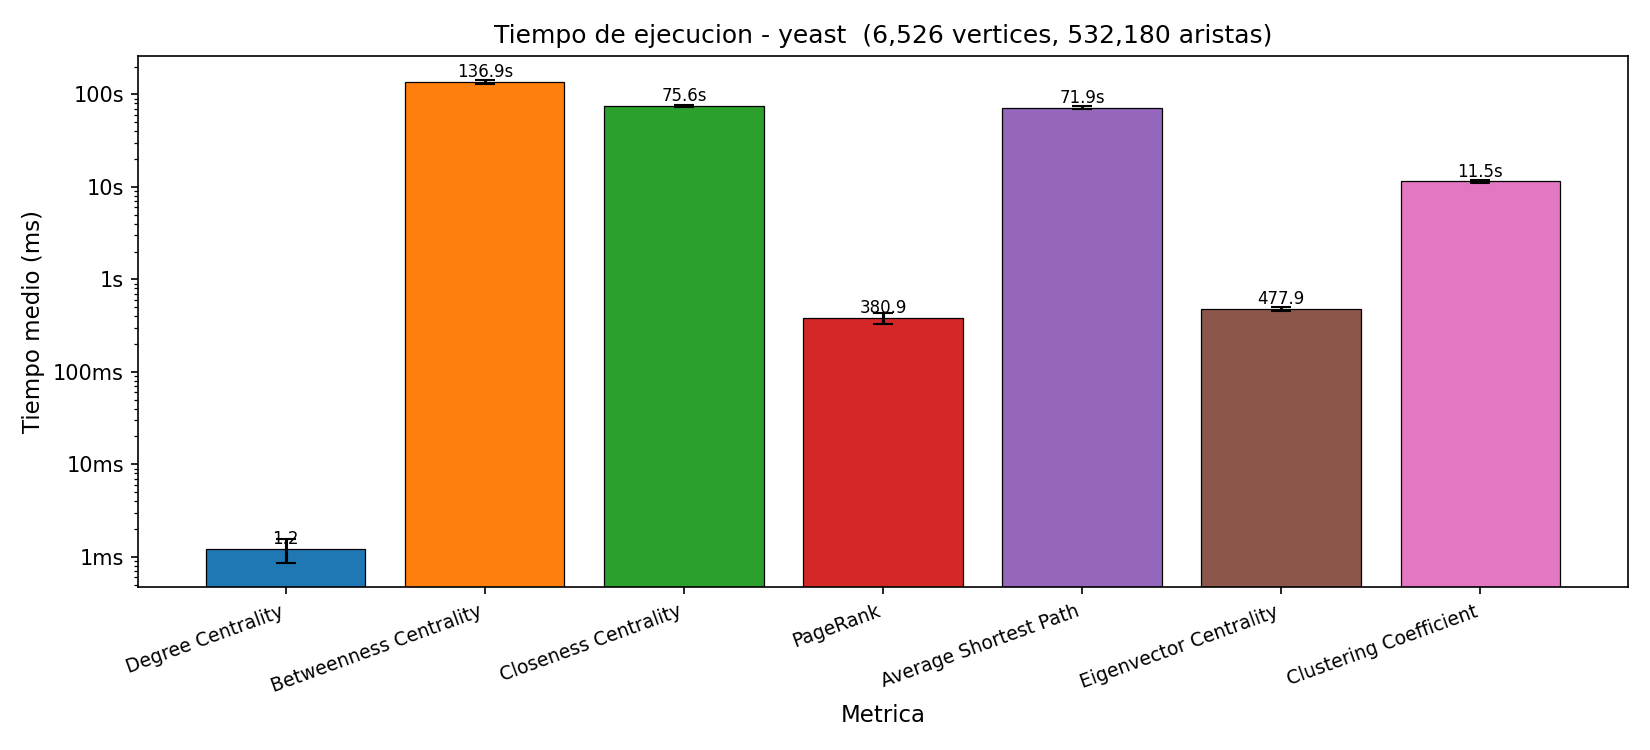
\includegraphics[width=0.48\textwidth]{../results/plots/yeast_tiempos.png}
\hfill
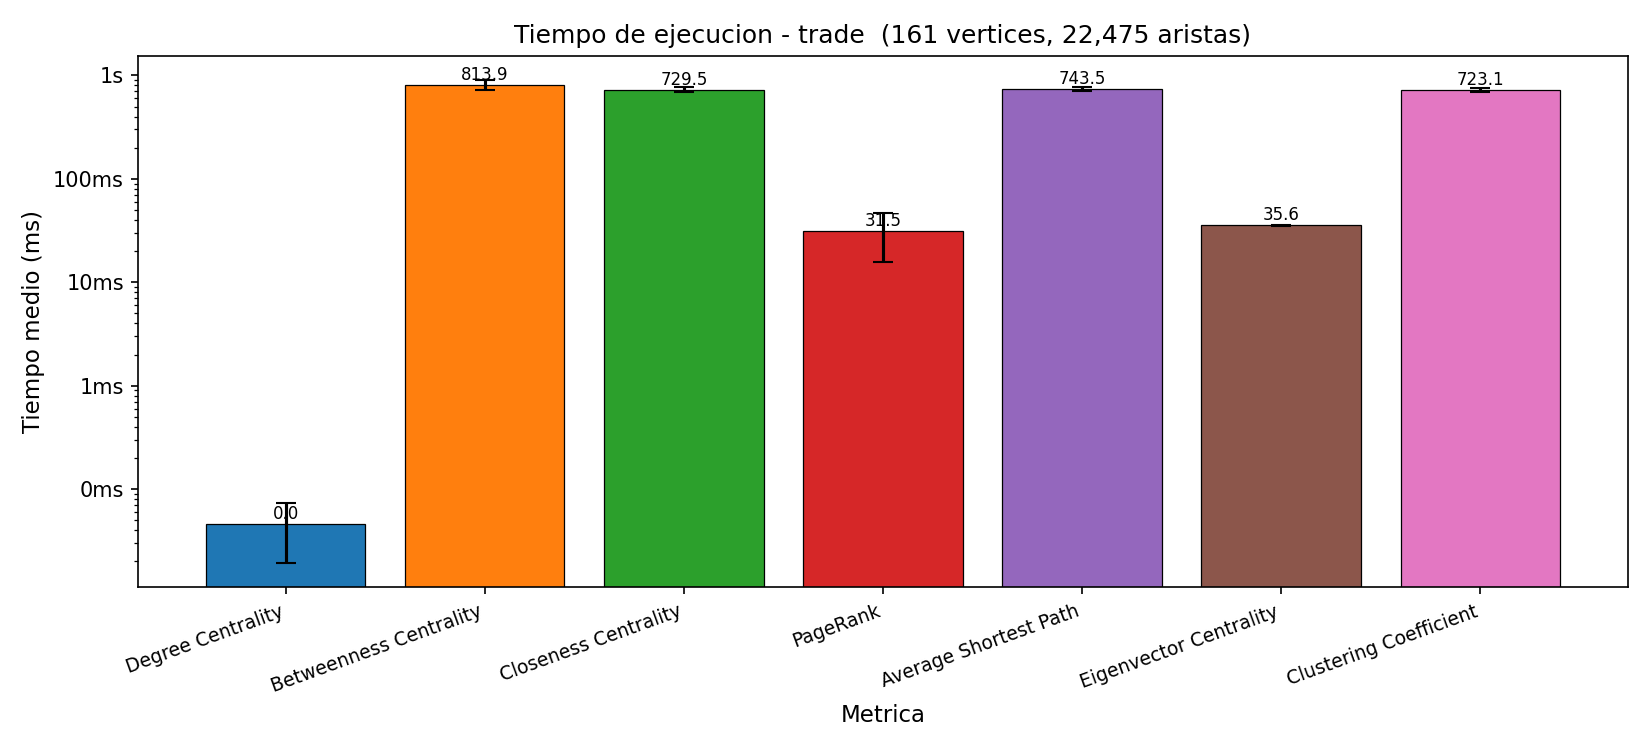
\includegraphics[width=0.48\textwidth]{../results/plots/trade_tiempos.png}
\caption{Tiempos de ejecución por métrica. Izquierda: Yeast PPI. Derecha: Trade Network.
Escala logarítmica para visualizar el rango de 6 órdenes de magnitud.}
\end{figure}

\subsection{Métricas Adicionales: Eigenvector y Clustering Coefficient}

\textbf{Eigenvector Centrality} tardó 411 ms en Yeast (varianza 178 ms$^2$) y 34,5 ms
en Trade (varianza 0,049 ms$^2$). La baja varianza en ambos datasets confirma que
Power Iteration converge de forma predecible en menos de 100 iteraciones.
En Yeast, los nodos con alta Eigenvector Centrality corresponden a proteínas que
interactúan con otras proteínas también muy conectadas, formando el núcleo funcional
de la red. En Trade, identifica países cuya influencia comercial se amplifica a través
de sus socios estratégicos.

\textbf{Clustering Coefficient} tardó 10.493 ms en Yeast (varianza 341 ms$^2$) y
699 ms en Trade (varianza 581 ms$^2$). La varianza es la más baja de las métricas
lentas, producto del comportamiento determinista del conteo de triángulos.
En Yeast, el alto coeficiente de clustering global indica la presencia de complejos
proteicos: módulos donde todas las proteínas interactúan entre sí (ribosomas, complejos
de transcripción). En Trade, países con alto clustering pertenecen a bloques comerciales
regionales donde sus socios también comercian entre sí.

\subsection{Impacto de Modificaciones Estructurales}

Se evaluó el impacto de agregar y quitar 5 aristas en tres zonas: nodos \textit{hub}
(top 10\% por grado), periféricos (bottom 10\%) y posiciones aleatorias.

\subsubsection*{Yeast PPI}

\begin{center}
\begin{tabular}{llccc}
\toprule
\textbf{Op.} & \textbf{Zona} & \textbf{Betweenness} & \textbf{Closeness} & \textbf{ASP} \\
\midrule
$+$5 & Hub        & $-4{,}3\times10^{-5}$\% & $+2{,}5\times10^{-5}$\% & $-2{,}3\times10^{-5}$\% \\
$+$5 & Periférico & $-0{,}007$\%             & $+0{,}003$\%             & $-0{,}004$\% \\
$+$5 & Aleatorio  & $-0{,}001$\%             & $+0{,}0004$\%            & $-0{,}0005$\% \\
\midrule
$-$5 & Hub        & $+5{,}0\times10^{-5}$\% & $-2{,}8\times10^{-5}$\% & $+2{,}8\times10^{-5}$\% \\
$-$5 & Periférico & $-0{,}158$\%             & $-0{,}060$\%             & $-0{,}082$\% \\
$-$5 & Aleatorio  & $-0{,}053$\%             & $-0{,}020$\%             & $-0{,}027$\% \\
\bottomrule
\end{tabular}
\end{center}

\subsubsection*{Trade Network}

\begin{center}
\begin{tabular}{llccc}
\toprule
\textbf{Op.} & \textbf{Zona} & \textbf{Betweenness} & \textbf{Closeness} & \textbf{ASP} \\
\midrule
$+$5 & Hub        & $0$\%        & $0$\%        & $0$\%      \\
$+$5 & Periférico & $+5{,}86$\%  & $+0{,}354$\% & $+1{,}135$\% \\
$+$5 & Aleatorio  & $-0{,}189$\% & $+0{,}013$\% & $-0{,}018$\% \\
\midrule
$-$5 & Hub        & $+0{,}189$\% & $-0{,}021$\% & $+0{,}018$\% \\
$-$5 & Periférico & $+0{,}189$\% & $-0{,}010$\% & $+0{,}018$\% \\
$-$5 & Aleatorio  & $+0{,}189$\% & $-0{,}017$\% & $+0{,}018$\% \\
\bottomrule
\end{tabular}
\end{center}

\subsection{Análisis de los Resultados}

\textbf{Betweenness domina en tiempo.} En Yeast tardó 109 segundos por ejecución,
representando más del 98\% del tiempo total del experimento. Esto confirma la
predicción teórica de $O(|V| \cdot |E|) \approx 3{,}47\times10^9$ operaciones.
El algoritmo de Brandes es indispensable: sin él, la complejidad naive
$O(|V|^2 \cdot |E|)$ haría el cálculo inviable.

\textbf{Closeness y ASP son equivalentes en tiempo.} Ambas realizan BFS desde
cada vértice, compartiendo la implementación \texttt{bfsDistances()}, lo que se
refleja en tiempos casi idénticos (60.020 ms vs 60.042 ms en Yeast).

\textbf{Diferencia de escala entre datasets.} Betweenness en Trade (722 ms) vs
Yeast (109.452 ms) — una diferencia de $\sim$150$\times$, consistente con la
relación entre sus tamaños ($|V|\cdot|E|$: Trade $\approx 3{,}6\times10^6$ vs
Yeast $\approx 3{,}5\times10^9$).

\textbf{Yeast es robusta ante cambios locales.} Con 532.180 aristas, agregar o
quitar 5 produce variaciones menores al 0,2\% en todas las métricas. Los cambios
son mayores en nodos periféricos que en hubs, ya que los hubs ya disponen de
múltiples caminos alternativos.

\textbf{Trade es sensible en su periferia.} Agregar 5 aristas desde nodos
periféricos aumenta Betweenness un 5,86\%, pues crea caminos mínimos nuevos que
reorganizan el flujo global. Los hubs, en cambio, muestran 0\% de cambio al agregar
aristas: con densidad $\approx 87\%$, ya no existen pares sin conexión entre los
nodos más conectados.

\section{Conclusiones}

Este proyecto implementó un sistema completo de análisis de redes en C++17,
cubriendo siete métricas de centralidad aplicadas a dos redes reales con
características contrastantes: una red biológica dispersa y de gran escala,
y una red económica densa y pequeña.

Los experimentos confirman que \textbf{la representación importa}: la lista de
adyacencia permite analizar Yeast con 24 MB frente a los 340 MB de una matriz,
diferencia determinante para la factibilidad del análisis.

\textbf{Betweenness es el cuello de botella computacional}. Su complejidad
$O(|V|\cdot|E|)$ implica 109 segundos por ejecución en Yeast. El algoritmo de
Brandes es la única razón por la que este cálculo es viable; sin él tomaría días.
En contraste, PageRank y Eigenvector convergen en menos de 100 iteraciones,
siendo eficientes incluso en la red más grande.

El experimento de aristas revela una diferencia estructural fundamental:
\textbf{Yeast es robusta} (alta densidad, cambios mínimos ante perturbaciones),
mientras que \textbf{Trade es sensible en su periferia} (nodos poco conectados
amplifican el impacto de cada arista nueva). En términos aplicados, esto sugiere
que en el comercio internacional, integrar economías periféricas tiene mayor impacto
estructural que reforzar vínculos entre potencias ya conectadas.

Las métricas adicionales aportan dimensiones complementarias: Eigenvector Centrality
captura la \textit{influencia propagada} (estar conectado a nodos importantes) y
Clustering Coefficient mide la \textit{cohesión local} (formación de grupos o módulos).
Juntas con las cinco métricas base, ofrecen una visión multidimensional de la
importancia de cada nodo que ninguna métrica individual puede proporcionar por sí sola.

\begin{thebibliography}{9}

\bibitem{brandes2001}
U. Brandes,
``A faster algorithm for betweenness centrality,''
\textit{Journal of Mathematical Sociology}, vol. 25, no. 2, pp. 163--177, 2001.
\newline\url{https://doi.org/10.1080/0022250X.2001.9990249}

\bibitem{pagerank1999}
L. Page, S. Brin, R. Motwani, T. Winograd,
``The PageRank Citation Ranking: Bringing Order to the Web,''
\textit{Stanford InfoLab Technical Report}, 1999.
\newline\url{https://www.cis.upenn.edu/~mkearns/teaching/NetworkedLife/pagerank.pdf}

\bibitem{wasserman1994}
S. Wasserman, K. Faust,
\textit{Social Network Analysis: Methods and Applications}.
Cambridge University Press, 1994.

\bibitem{cormen2009}
T. H. Cormen, C. E. Leiserson, R. L. Rivest, C. Stein,
\textit{Introduction to Algorithms}, 3rd ed.
MIT Press, 2009.

\bibitem{bonacich1987}
P. Bonacich,
``Power and Centrality: A Family of Measures,''
\textit{American Journal of Sociology}, vol. 92, no. 5, pp. 1170--1182, 1987.
\newline\url{https://web.archive.org/web/20210729125432id_/http://www.leonidzhukov.net/hse/2014/socialnetworks/papers/Bonacich-Centrality.pdf}

\bibitem{watts1998}
D. J. Watts, S. H. Strogatz,
``Collective dynamics of `small-world' networks,''
\textit{Nature}, vol. 393, pp. 440--442, 1998.
\newline\url{https://snap.stanford.edu/class/cs224w-readings/watts98smallworld.pdf}

\end{thebibliography}


\end{document}
